\section{PROBLEMS DETECTED AND SOLUTIONS IMPLEMENTED}
\label{problems}

\subsection{Memory limits}
As several software resources for the \acrshort{lorawan} stack were used, The amount of \acrfullr{ram} used by the system was more than the previous project without the measurement threads.

When the system was being tested, and the threads included in the project, the call to start the threads returned an \texttt{osStatus==osErrorNoMemory(0x85)}. This indicated that the 
\acrfullr{rtos}  could not allocate the stack size indicated in the constructor call for the thread.

Another factor that worsen the issue was the queue developed for the communication of the previous project. This queue needed the allocation of 
more bytes to be able to manage more structures. In reaction to this, the communication decision to use only 1 structure with a mutex was done.

Following the problems with the threads, to further understand the requirements of memory to adjust the stack size for each thread, a stack tracing tool was used\cite{Runtimememorystatistics}.

With this tool, the results in \autoref{fig:memstack} were achieved in terms on stack analysis.
\begin{figure}[H]
    \centering
    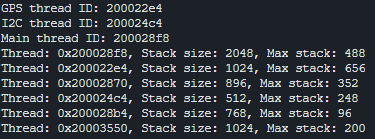
\includegraphics[width=0.7\textwidth]{images/7/Thread Traced.png}
    \caption{Threads stack usage for problem detection}
    \label{fig:memstack}
\end{figure}

As can be seen in the figure, ignoring the main thread that is not supposed to be changed, the \acrfullr{i2c} thread only uses around \texttt{248 Bytes}, while the GPS thread uses around \texttt{656 Bytes}(this is the result of the parsing of \acrfullr{nmea} data).

With this in mind, the stack were defined as follows: \texttt{512 Bytes} for the \acrshort{i2c} thread and \texttt{1024 Bytes} for the GPS thread.

\subsection{Frame size limits}

The \acrshort{lorawan} technology used in this project only allows around $1\%$ duty cycle in Europe. Because of this, it is very important for the application to use all the bits of the application message as much as possible. This allows for higher relation between transmitting windows allocation and information exchanged between the node and the network server.

In the case of the project, the frame size is \texttt{30 Bytes}, and at the start of the project, sending all the data in one single frame seemed impossible without trunking float values, which results in loss of precision.

As the user sees a lot of values that are only important as percentage, a encoding to metrics such as humidity, light and moisture was designed:
\begin{enumerate}
    \item The value is processed in the \acrfullr{mcu}, which gives a float \% value from \texttt{0.0} to \texttt{100.0} .
    \item Then, the value is multiplied by 10 and converted to an unsigned integer.
    \item Finally, as the value goes from \texttt{0} to \texttt{1000}, it can be expressed with only \texttt{10 bits}.
    \item When received in the network server, the value can be divided by 10 and we have a percentage value with at least 1 decimal, which is perfect for this use case. 
    This approach only reduces precision percentage values without trunking, while leaving full precision for the acceleration.
\end{enumerate}

This encoding gave enough room to send all the data in \texttt{29 Bytes}, and allowed the inclusion of a header byte in the frame.

\subsection{Usage of LUA 5.1}

The design solution for the frame described above created another problem in the Network Server. The Network Server script 
uses \texttt{LUA 5.1,} which doesn't support the most important bitwise operators\cite{luauserswikiBitwise} such as shifting.

To solve this, the next steps were taken:
\begin{enumerate}
    \item All the values that were align were send first on the frame structure.
    \item As the frame had a moment in which the byte alignment was lost, it was decided to separate acceleration values to make \texttt{3 Byte} combinations between one percentage 
    value and one acceleration axis. This meant that the bit masking and shifting operation needed to be designed once.
    \item Then, the values were obtained using the function that the ResIoT library provides and simple divisions.
\end{enumerate}
